\begin{task}{1, Introduction of approach and dataset (15\%)}
In this project we will implement, test and compare neural networks and knowledge-based approaches in the context of pedestrian dynamics. 

The project is mainly based on two papers: \textit{Prediction of Pedestrian Dynamics in Complex Architectures with Artificial
Neural Networks} \cite{tordeux2020prediction}, where the authors use neural networks to predict the velocity of crowds in different scenarios and compare them to a simple knowledge-based approach, and \textit{Review of Pedestrian Trajectory Prediction Methods: Comparing Deep
Learning and Knowledge-based Approaches} \cite{korbmacher2022review}, where an in-depth comparison between the two approaches is done, highlighting the pros and drawbacks of both of them.

In this task, we will explain the knowledge-based (with a focus in the speed-based model we are using) and the neural network approaches in more detail. Furthermore, we will define and review the dataset we will use to test and compare these models in a fair way.

\paragraph{Knowledge-based models}
Knowledge-based models are characterized by a defined set of rules or equations that take into account various factors such as physical, social, or psychological aspects of pedestrians. These models are typically described by a small number of parameters with clear physical interpretations, facilitating adjustments to the model. 

Currently, knowledge-based models span macroscopic, mesoscopic, and microscopic scales, each addressing specific characteristics of the modeling scale. Macroscopic and mesoscopic approaches borrow concepts from continuous fluid dynamics or gas-kinetic models, providing an aggregated description of dynamics \cite{henderson1971statistics}, \cite{henderson1974fluid}. On the other hand, microscopic approaches focus on modeling individual pedestrian motions. Researchers have extensively explored microscopic models, emphasizing the advantage of capturing heterogeneous behaviors due to their ability to individually represent pedestrians. This allows for the attribution of specific characteristics to each agent, considering behavioral heterogeneity and other diverse aspects. 

In our previous projects and the current one, we have employed the microscopic approach within knowledge-based models. Therefore, our explanation from now on will focus on this particular subset of models.

These models, which describe individual pedestrian dynamics, are versatile in predicting pedestrian trajectories at any scale. By providing input information like the initial position, velocity, and acceleration of pedestrians, a forward simulation using these rules can forecast future trajectories.

The way the pedestrian motion to a new position is determined depends on the model's inputs and outputs. If the model outputs new velocity or acceleration, enabling the calculation of the new position, it is classified as a velocity- or acceleration-based model. Alternatively, if the position is directly determined by specific rules without involving differential equations, the models fall into the category known as decision-based (e.g. cellular automata).

Finally, we will focus on speed-based models, in particular, the one we will use in this project. Based on \cite{tordeux2020prediction} we will implement and test a speed-based model to compare them to the neural networks. As in the paper, the goal is to predict the speed of pedestrians based on their positions and, if available, the velocity of their K closest neighbors. In the context of this description, \((x, y)\) represents the position of the considered agent, \(v\) indicates its speed, while \((x_i, y_i)\) for \(i = 1, ..., K\) and \((v_i, u_i)\) for \(i = 1, ..., K\) denote the positions and velocities of the K closest neighbors, respectively. 

The  modelling approach is the parametric Weidmann fitting model \cite{weidmann1993transporttechnik}. In this model, the speed is represented as a non-linear function of the mean spacing, characterized by three parameters as:
\begin{align}
    W&(\overline{s}_K, v_0, T, l) = v_0\cdot\left(1-e^{\frac{l-\overline{s}_K}{v_0 T}}\right)\label{exp_tor}\\
    \overline{s}_K &= \frac{1}{K}\sum_i\sqrt{(x-x_i)^2 + (y-y_i)^2}\label{exp_mean}
\end{align}
where \(\overline{s}_K\) is the mean Euclidian spacing to the K closest neighbors. The time gap parameter T
corresponds to the following time gap with the neighbors, \(v_0\) is the speed of pedestrians
in a free situation while \(l\) describes the physical size of a stopped pedestrian. 

This model will be implemented and tested in Task 3.

\paragraph{Deep learning}
Deep learning involves training neural networks with more than two hidden layers. In this approach we rely on big amounts of data to learn the underlying dynamics of the pedestrians. In contrast to the knowledge-based approach, in the deep learning framework we do not need to design a set of rules or functions that aligns with the real dynamics of pedestrians, we obtain the function implicitly by training on the data of past trajectories. Also, neural networks' parameters are non-interpretable (weights), i.e. they lack of a physical interpretation like in the Weidmann model \cite{korbmacher2022review}.

In this section, we will present the basic neural network model that we plan to build in Task 2. Drawing inspiration from the approach outlined in \cite{tordeux2020prediction}, we intend to employ feed-forward artificial neural networks for predicting pedestrian speed. Our strategy involves experimenting with different architectures characterized by varying numbers of hidden layers denoted as \textit{h}. In \cite{tordeux2020prediction} they use 4 different types of combination of inputs parameters. However, we will use only the one that achieved the best results in the paper. This is because our project is more focused in comparing the two approaches, so we do not need the ones that performed badly. The neural networks are designed to produce predictions of pedestrian speed based on a given set of input parameters: The network we use depends on the relative positions and also the mean distance spacing \(\bar{s}_K\) to the K closest neighbors (2K + 1 inputs):
    \[
    NN_3 = NN_3(\bar{s}_K, (x_i - x, y_i - y, 1 \le i \le K))
    \]
This one corresponds to network definition \(NN_3\) in \cite{tordeux2020prediction}.

We will see in Task 2 that it was difficult to replicate the results of this paper. Therefore, we divided our efforts: \textbf{Task 2 is divided into two parts}. One focusing in a data-centric approach, and the other one focusing on exploring different types of architectures.

\paragraph{Dataset introduction}
To train, test and compare the models, we will use the dataset detailed in \cite{keip2009dokumentation}. The dataset consists of trajectories of pedestrians in two different scenarios: The \textit{Bottleneck} and the \textit{Corridor}. 

Independently of the scenario, each data row is composed by 5 columns:
\begin{itemize}
    \item ID of the pedestrian
    \item Frame number (frame rate is 1/16s)
    \item X coordinate
    \item Y coordinate
    \item Z coordinate
\end{itemize}

The corridor data comprises trajectories of pedestrians moving within a closed corridor with a length of 30m and a width of 1.8m. The trajectories are recorded over a specific section measuring 6m. The experiments involve varying participant numbers, specifically N=15, 30, 60, 85, 95, 110, 140, and 230. The experiments in this scenario are named with the prefix \textit{UG}.

As for the bottleneck data, it consists of trajectories of pedestrians navigating through a bottleneck with a length of 8m and a width of 1.8m. The experiments in this case are conducted with 150 participants, exploring different bottleneck widths: w=0.7, 0.95, 1.2, and 1.8m. The experiments in this scenario are named with the prefix \textit{UO}.
\begin{figure}[H]
\centering
\subfigure[Corridor experiment (UG)]{
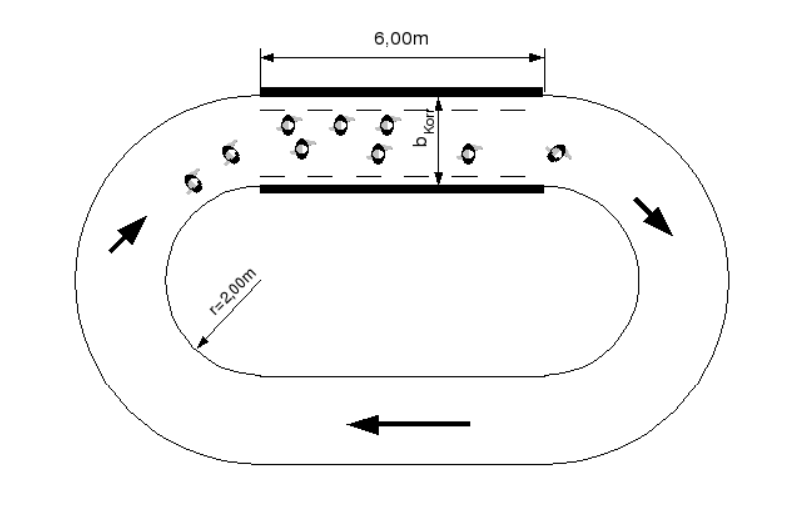
\includegraphics[width=0.5\textwidth]{images/corridor.png}\label{scenarioa}}
\subfigure[Bottleneck experiment (UO)]{
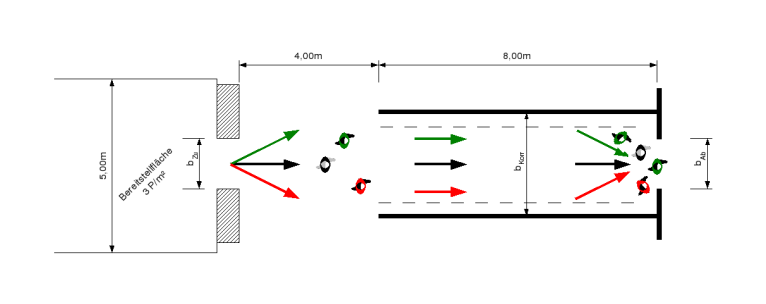
\includegraphics[width=0.5\textwidth]{images/bottleneck.png}\label{scenariob}}
\caption{Scheme of scenarios in the dataset}
\label{scenario}
\end{figure}

After providing an overview of the dataset, we proceed with an initial analysis. This analysis can be found in the notebook \verb|data_visualization.ipynb|, that uses the functions in \verb|utils/data_processing.py| and \verb|utils/visualization.py|. The details about which code is related to each task can be easily found in the \verb|README.md| in the repository.

Initially, it is important to note that the trajectories are three-dimensional, as the Z coordinate represents the height of each pedestrian. Considering the potential complexity introduced by the Z coordinate, we conduct tests to ensure if it indeed contributes relevant information.

Upon investigation, it was determined that the Z coordinate remains constant for each pedestrian throughout the observed time period. This can be visualized in Figure \ref{z_not_changing}, where the Z coordinates of four randomly selected pedestrians are plotted over time for each experiment in both scenarios. Each colored line represents the Z coordinate for a specific ID in a given experiment.
\begin{figure}[H]
\centering
\subfigure[Corridor experiments Z coordinate]{
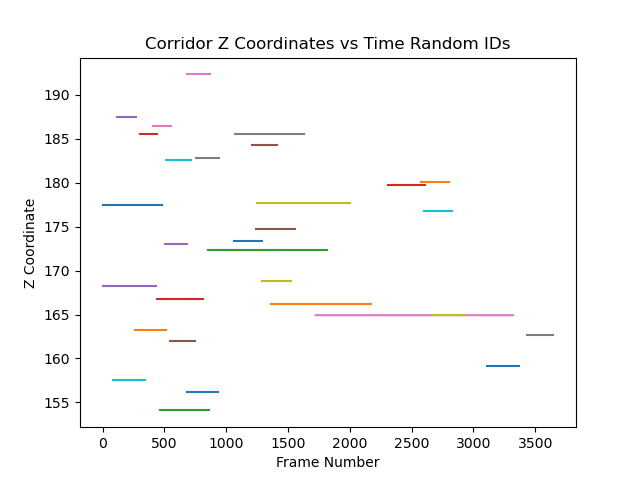
\includegraphics[width=0.45\textwidth]{images/Corridor Z Coordinates vs Time Random IDs.png}\label{z_not_changinga}}
\subfigure[Bottleneck experiments Z coordinate]{
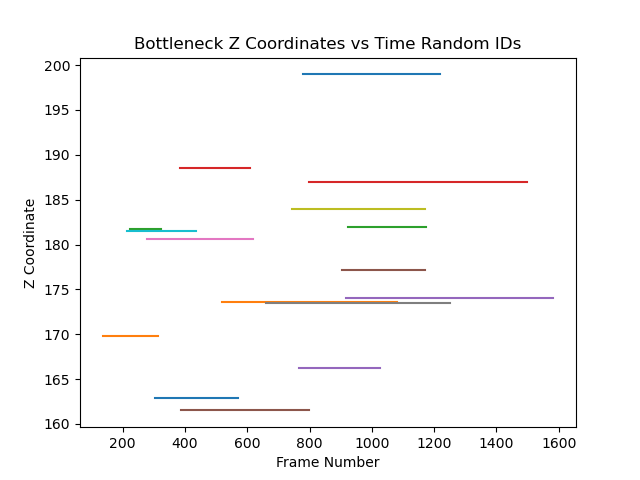
\includegraphics[width=0.45\textwidth]{images/Bottleneck Z Coordinates vs Time Random IDs.png}\label{z_not_changingb}}
\caption{Z coordinate against the time}
\label{z_not_changing}
\end{figure}

Due to this lack of change in the Z coordinate, we will not use it for our computations in the following tasks.

After this, we can visualize the trajectories data (i.e. the X and Y coordinates). In Figure \ref{vistraj} we can observe different experiments for each type of scenario. We highlight in black the two trajectories made for pedestrians with ID 1 and 2 for better understanding of the plot. The trajectories of the chosen pedestrians progress from black to white.
\begin{figure}[H]
\centering
\subfigure[Bottleneck experiment with width = 0.7m]{
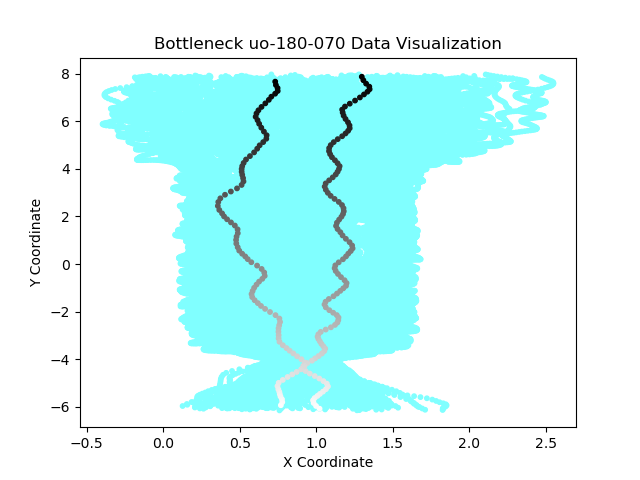
\includegraphics[width=0.45\textwidth]{images/Bottleneck_uo-180-070_visualization.png}\label{vistraja}}
\subfigure[Bottleneck experiment with width = 1.2m]{
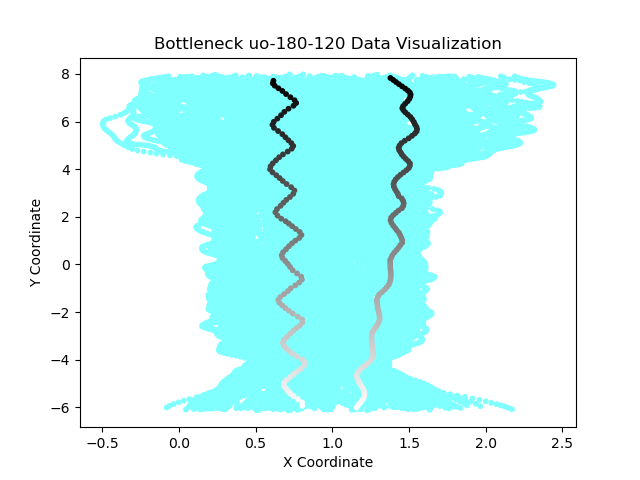
\includegraphics[width=0.45\textwidth]{images/Bottleneck_uo-180-120_visualization.png}\label{vistrajb}}
\subfigure[Bottleneck experiment with width = 1.8m]{
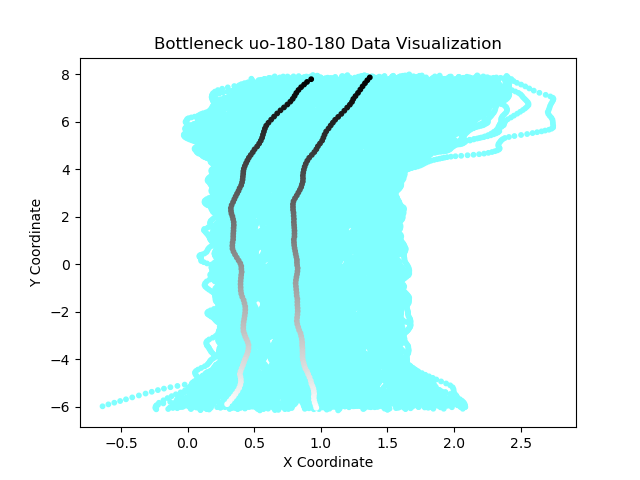
\includegraphics[width=0.45\textwidth]{images/Bottleneck_uo-180-180_visualization.png}\label{vistrajc}}
\subfigure[Corridor experiment with N = 30]{
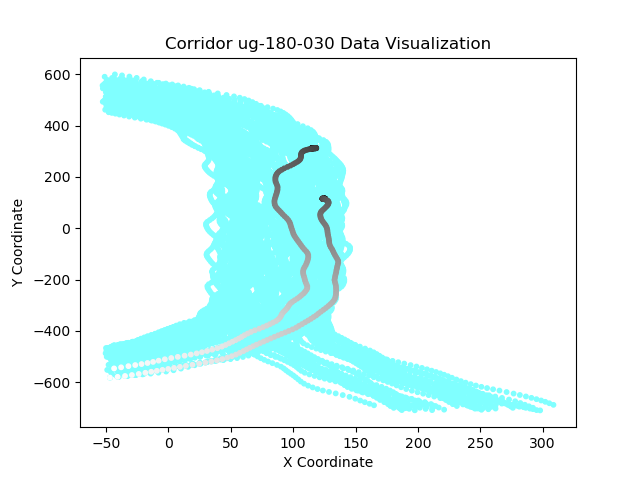
\includegraphics[width=0.45\textwidth]{images/Corridor_ug-180-030_visualization.png}\label{vistrajd}}
\subfigure[Corridor experiments with N = 95]{
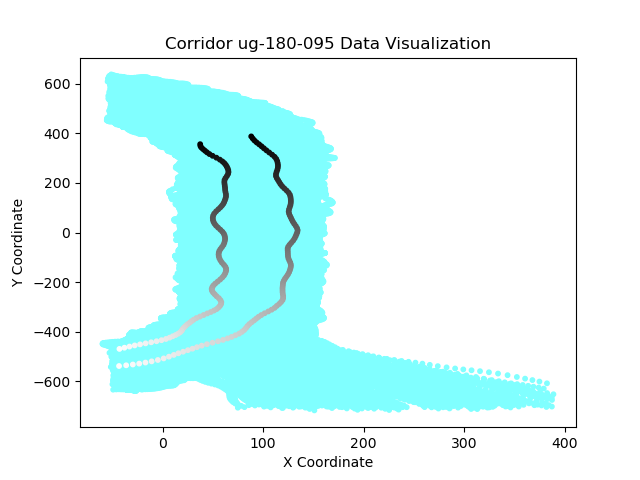
\includegraphics[width=0.45\textwidth]{images/Corridor_ug-180-095_visualization.png}\label{vistraje}}
\subfigure[Corridor experiments with N = 230]{
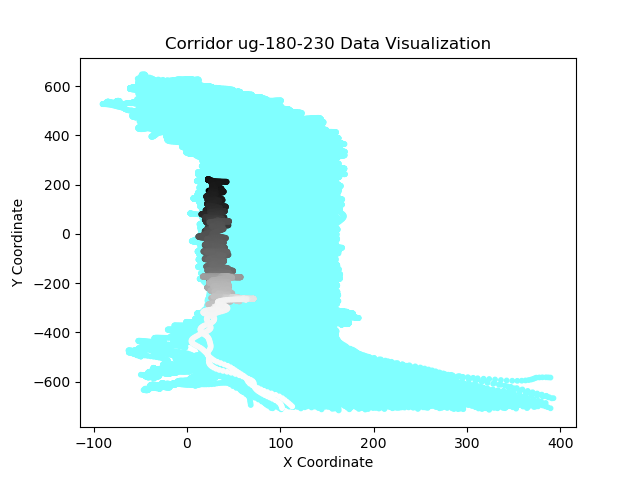
\includegraphics[width=0.45\textwidth]{images/Corridor_ug-180-230_visualization.png}\label{vistrajf}}
\caption{Trajectories in different experiments}
\label{vistraj}
\end{figure}

Comparing figures \ref{vistraja}, \ref{vistrajb} and \ref{vistrajc}, it is evident that the augmented bottleneck width, compared to the previous experiment, leads to trajectories being less closely spaced within the bottleneck. In the corridor scenario, a comparison of Figures \ref{vistrajd}, \ref{vistraje}, and \ref{vistrajf} shows that as the number of pedestrians increases, the number of trajectories also rises. Additionally, in Figure \ref{vistrajf} the trajectories become more clustered and exhibit an apparent reduced speed, likely due to the higher volume of people in the corridor.
\end{task}